\documentclass{article}
\usepackage[utf8]{inputenc}
\usepackage{polski}
\usepackage[lined,boxed]{algorithm2e}
\usepackage{float}
\usepackage{graphicx}
\title{Sprawozdanie}
\author{Kajetan Bilski 244942}

\begin{document}
	\maketitle
	\pagenumbering{arabic}

\section{Zadanie 1.}
W tym zadaniu trzeba zaimplementować funkcję liczącą ilorazy różnicowe funkcji na podstawie jej wartośći w wybranych punktach według podanej specyfikacji. Algorytm liczący nie może wykorzystywać macierzy (tablicy dwuwymiarowej).\\
Kody do zadań 1 - 4 są w pliku zad1234.jl, a testy do nich w testy.jl.\\
Pseudokod funkcji:\\
\begin{algorithm}[H]
$n \leftarrow length(x)$\\
\For{$i \leftarrow 1$ \KwTo $n$}{
	$r[i] \leftarrow f[i]$\\
	\For{$k \leftarrow 1$ \KwTo $i-1$}{
		$r[i-k] \leftarrow \frac{r[i-k+1]-r[i-k]}{x[i]-x[i-k]}$}
	$fx[i]\leftarrow r[1]$}
\KwRet $fx$\\
\end{algorithm}
W trakcie wykonywania się tablica $r$ "przesuwa się" po kolejnych przekątnych macierzy trójkątnej normalnie używanej do liczenia ilorazów różnicowych. W ten sposób rekurencyjna metoda liczenia jest zachowana, ale zmniejszamy złożoność pamięciową używając tablicy o maksymalnym rozmiarze $n$ zamiast macierzy.
\section{Zadanie 2.}
W tym zadaniu trzeba napisać według specyfikacji funkcję liczącą wartości wielomianu interpolacyjnego, która za argumenty przyjmuje punkty $x$, ilorazy różnicowe dla tych punktów i punkt w którym szukamy wartości. Funkcja ma być implementacją algorytmu Hornera z zadania 8. z listy 4. na ćwiczenia i mieć złożoność czasową $O(n)$.\\
Kody do zadań 1 - 4 są w pliku zad1234.jl, a testy do nich w testy.jl.\\
Pseudokod funkcji:\\
\begin{algorithm}[H]
$n \leftarrow length(x)$\\
$nt\leftarrow fx[n]$\\
\For{$i \leftarrow 1$ \KwTo $n-1$}{
	$nt \leftarrow (t-x[n-i])*nt+fx[n-i]$}
\KwRet $nt$
\end{algorithm}
Jak widać mamy tylko jedną pętlę wykonującą się $n-1$ razy, czyli złożoność czasowa to $O(n)$. Funkcja jest bezpośrednią implementacją algorytmu Hornera z listy na ćwiczenia.
\section{Zadanie 3.}
W tym zadaniu trzeba zaimplementować funkcję wyliczającą współczynniki postaci naturalnej wielomianu interpolacyjnego w czasie $O(n^2)$, mając punkty $x$ i jego ilorazy różnicowe dla tych punktów.\\
Kody do zadań 1 - 4 są w pliku zad1234.jl, a testy do nich w testy.jl.\\
Pseudokod funkcji:\\
\begin{algorithm}[H]
$n \leftarrow length(x)$\\
\emph{$a$ jest tablicą $n$ zer}\\
$a[n] \leftarrow fx[n]$\\
\For{$i \leftarrow 1$ \KwTo $n-1$}{
	$a[n-i] \leftarrow fx[n-i]$\\
	\For{$k \leftarrow n-i$ \KwTo $n-1$}{
		$a[k] \leftarrow a[k]-x[n-i]*a[k+1]$}}
\KwRet $a$
\end{algorithm}
Jak widać mamy dwie pętle, których łączny czas wykonania jest $O(n^2)$. Funkcja zaczyna od współczynnika $a_n$ który jest równy $f[x_0,...,x_n]$. Potem funkcja dodaje koolejne punkty $x$ i ilorazy różnicowe o malejących indeksach. W każdej iteracji i pętli dodawany jest współczynnik $a_{n-i}=fx[n-i]$ i akualizowane są wszystkie dotychczasowe współczynniki z użyciem $x_{n-i}$.
\section{Zadanie 4.}
W tym zadaniiu trzeba zaimplementować funkcję, która dla zadanej funkcji stworzy przybliżający ją wielomian interpolacyjny dla $n+1$ punktów w przedziale $[a,b]$, a następnie narysuje je obok siebie na wykresie używając funkcji z zadań 1 i 3.\\
Kody do zadań 1 - 4 są w pliku zad1234.jl, a testy do nich w testy.jl.\\
Pseudokod funkcji:\\
\begin{algorithm}[H]
$h \leftarrow (b-a)/n$\\
\For{$i \leftarrow 0$ \KwTo $n$}{
	$x_i \leftarrow a+i*h$\\
	$y_i \leftarrow f(x_i)$}
$fx \leftarrow$ \verb|ilorazyRoznicowe(|$x$,$y$\verb|)|\\
\emph{Następnie funkcja nakłada na wykres na przedziale $z\in[a,b]$ funkcje $f(z)$ i $warNewton(x,fx,z)$.}
\end{algorithm}
Funkcji ilorazyRoznicowe używam do znalezienia ilorazów różnicowych, potrzebnych dla funkcji warNewton, której używam do wyznaczania wartości wielomianu interpolacyjnego.
\section{Zadanie 5.}
W tym zadaniu trzeba użyć funkcji \verb|rysujNnfx| żeby narysować wykresy z podanymi danymi.
Kod w pliku zad5.jl.
\begin{figure}[H]
	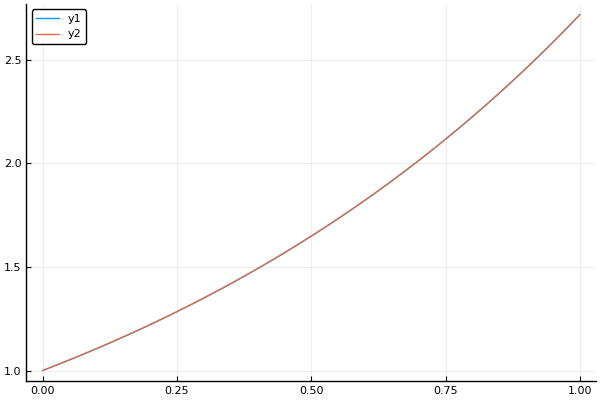
\includegraphics[width=\linewidth]{zad5a_5.png}
	\caption{$f(x) = e^x$, $[a,b]=[0,1]$, $n=5$}
	\label{fig:5a5}
\end{figure}
\begin{figure}[H]
	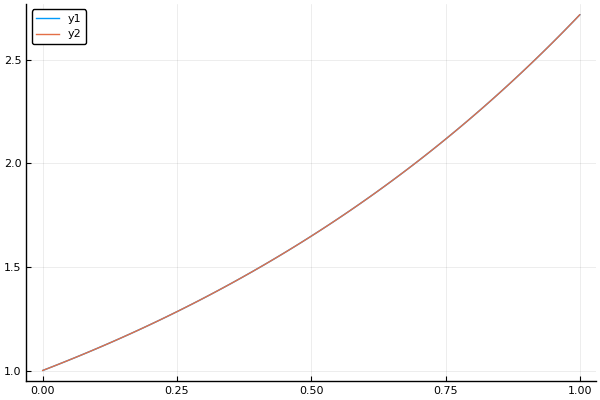
\includegraphics[width=\linewidth]{zad5a_10.png}
	\caption{$f(x) = e^x$, $[a,b]=[0,1]$, $n=10$}
	\label{fig:5a5}
\end{figure}
\begin{figure}[H]
	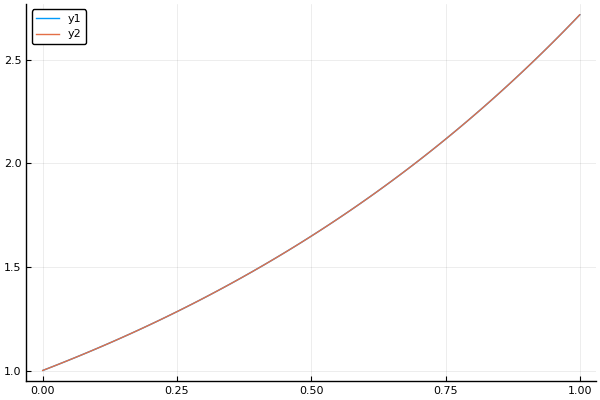
\includegraphics[width=\linewidth]{zad5a_15.png}
	\caption{$f(x) = e^x$, $[a,b]=[0,1]$, $n=15$}
	\label{fig:5a5}
\end{figure}
\begin{figure}[H]
	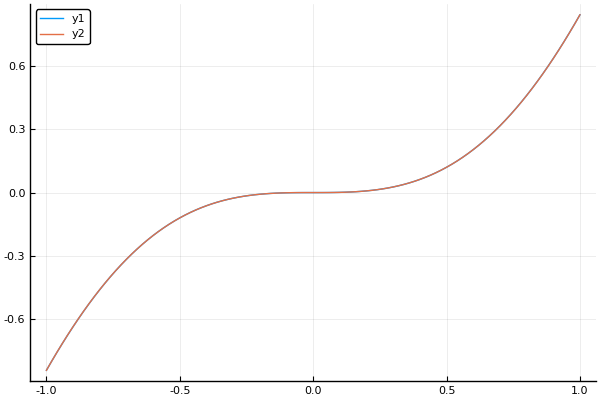
\includegraphics[width=\linewidth]{zad5b_5.png}
	\caption{$f(x) = x^2 sin x$, $[a,b]=[-1,1]$, $n=5$}
	\label{fig:5a5}
\end{figure}
\begin{figure}[H]
	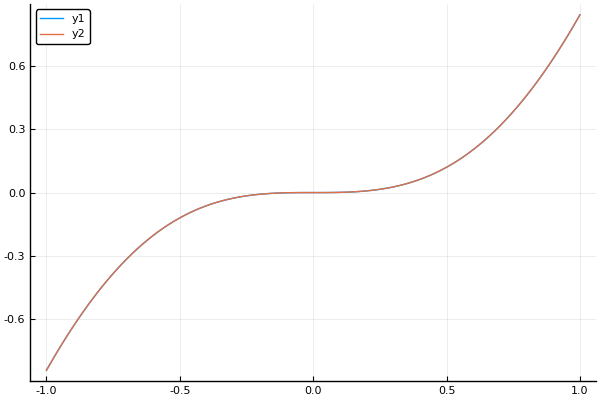
\includegraphics[width=\linewidth]{zad5b_10.png}
	\caption{$f(x) = x^2 sin x$, $[a,b]=[-1,1]$, $n=10$}
	\label{fig:5a5}
\end{figure}
\begin{figure}[H]
	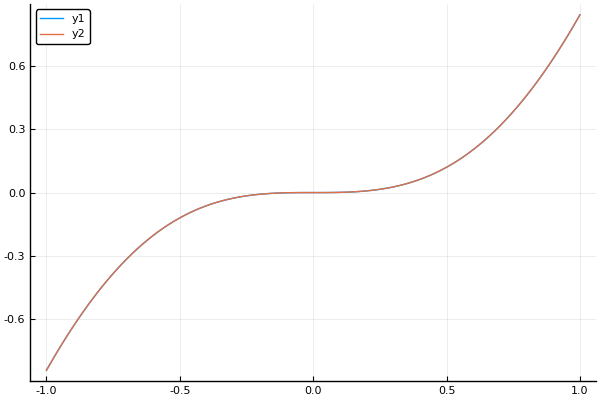
\includegraphics[width=\linewidth]{zad5b_15.png}
	\caption{$f(x) = x^2 sin x$, $[a,b]=[-1,1]$, $n=15$}
	\label{fig:5a5}
\end{figure}
Jak widać wielomiany interpolacyjne bardzo dobrze przybliżają dane funkcje na odpowiednich przedziałach. Nie ma widocznych różnic.
\section{Zadanie 6.}
W tym zadaniu trzeba zrobić to samo co w poprzednim, tylko z innymi danymi.
Kod w pliku zad6.jl.
\begin{figure}[H]
	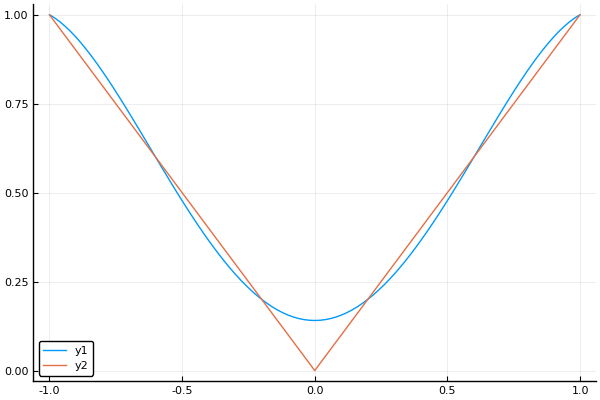
\includegraphics[width=\linewidth]{zad6a_5.png}
	\caption{$|x|$, $[a,b]=[-1,1]$, $n=5$}
	\label{fig:5a5}
\end{figure}
\begin{figure}[H]
	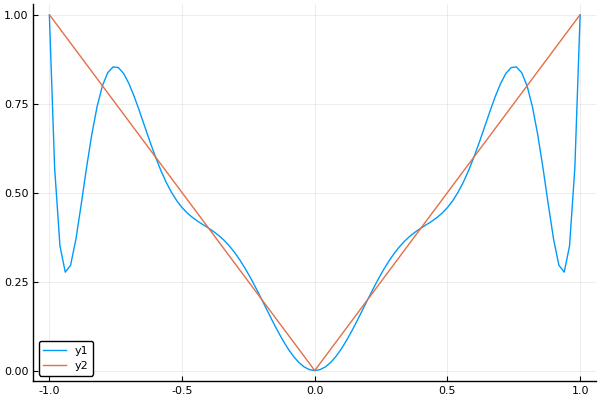
\includegraphics[width=\linewidth]{zad6a_10.png}
	\caption{$|x|$, $[a,b]=[-1,1]$, $n=10$}
	\label{fig:5a5}
\end{figure}
\begin{figure}[H]
	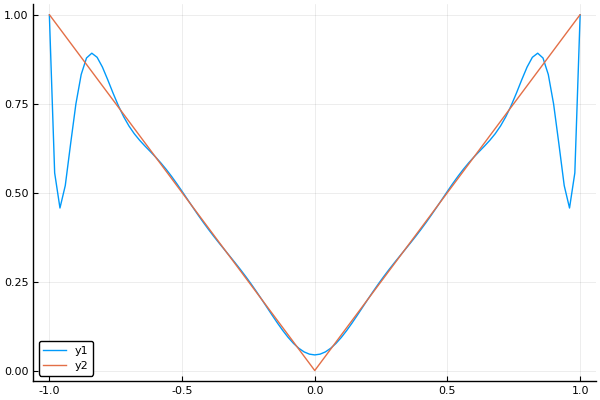
\includegraphics[width=\linewidth]{zad6a_15.png}
	\caption{$|x|$, $[a,b]=[-1,1]$, $n=15$}
	\label{fig:5a5}
\end{figure}
\begin{figure}[H]
	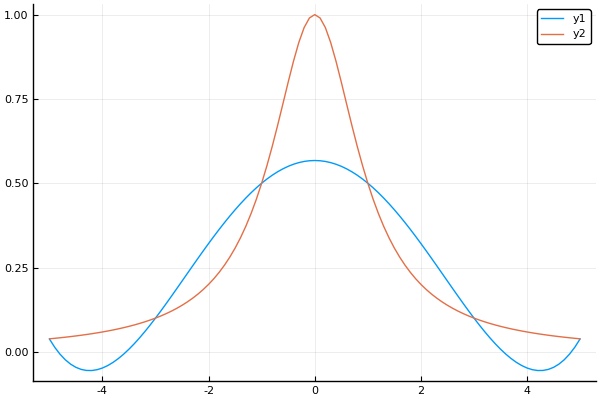
\includegraphics[width=\linewidth]{zad6b_5.png}
	\caption{$\frac{1}{1+x^2}$, $[a,b]=[-5,5]$, $n=5$}
	\label{fig:5a5}
\end{figure}
\begin{figure}[H]
	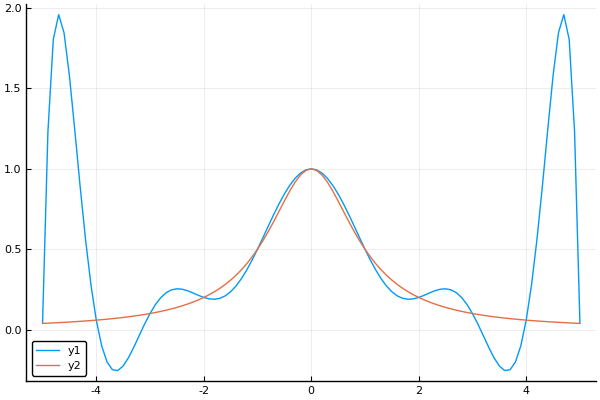
\includegraphics[width=\linewidth]{zad6b_10.png}
	\caption{$\frac{1}{1+x^2}$, $[a,b]=[-5,5]$, $n=10$}
	\label{fig:5a5}
\end{figure}
\begin{figure}[H]
	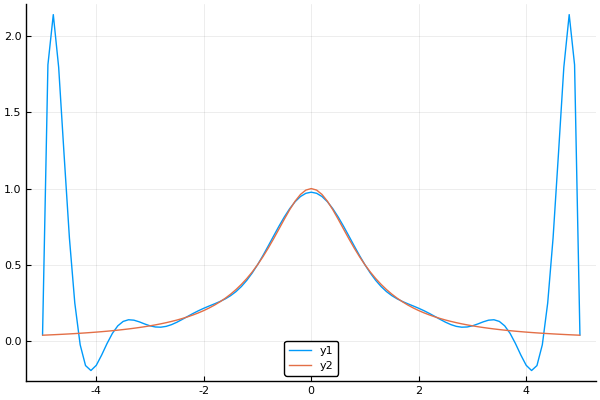
\includegraphics[width=\linewidth]{zad6b_15.png}
	\caption{$\frac{1}{1+x^2}$, $[a,b]=[-5,5]$, $n=15$}
	\label{fig:5a5}
\end{figure}
W tym zadaniu mocno widać pojawienie się efektu Rungego, czyli pogorszenia się jakości interpolacji wielomianowej pomimo zwiększenia liczby jej węzłów. Jest to szczególnie widoczne na końcach przedziału.
\end{document}